\documentclass[../../../main.tex]{subfiles}

\begin{document}
\label{sec:committee_service}

In 2017, my department had arranged my schedule such that I did not serve on a committee for the first year.  By Fall 2018, I had developed the idea that I could serve Whittier College through data analysis.  I was interested in the connection between the high school preparation of our students and their ability to pass introductory courses required for their major.  On the Enrollment and Student Affairs Committee (ESAC), in Fall 2018, I learned that this is a topic with which many administrators and intructors had been struggling.  I spent two years working on ESAC, and I watched as our committee carefully approached consensus while remaining respectful of the diverse perpectives that included athletics, student life, and instructors.  In the second year, we began discussions with Falone Serna, Vice President of Enrollment Management, to implement the policy result of the prior year.  On ESAC, I also learned about first year orientation, for which I volunteered in 2019 and 2020.
\\
\vspace{0.15cm}
In 2020-21, having served two years on ESAC, we decided it would be good for me to experience service with other types of committees.  I had taken an interest in the Digital Liberal Arts, and educational technology, after writing my Cottrell Scholars Grant\footnote{Provided in supporting material.}.  I decided to join the Educational Resources and Digital Liberal Arts Committee (ERC/DLAC) for a year.  Though the onset of the pandemic restricted our ability to procure educational resources, we studied the curriculum proposals and then decided to create two new initiatives.  The first initiative was to participate in the creation of a Center for Teaching and Learning.  The second was to create a policy for archival of all undergraduate senior projects in the Poet Commons.

\subsection{Enrollment and Student Affairs Committee, Years 1 and 2}

The charge given to ESAC in 2018 included the creation of recommendations for altering admissions criteria, discussing the criteria for athletics participation for students on probation, and organizational issues surrounding the creation of INTD101.  Our committee chair was Prof. Ayesha Shaikh.  Early in the year, Prof. Shaikh formed a sub-committee on admissions data analysis.  I volunteered to partipate with Prof. Charles Hill, and the vice president of enrollment (at the time) Kieron Miller was also included.  Working with Fritz Smith and others, we gathered educational data on thousands students.  The task was to examine what leads to the admission of students that do not proceed to their sophomore year.
\\
\vspace{0.25cm}
The admissions data sub-committee began meeting in Fall 2018.  Our discussions were broad at first, focusing on the the balance between admitting enough students with the need to admit students we know we can support and retain.  I learned a lesson about management: adminstrators and instructors more experienced than me spoke more frankly in sub-committee, but in more diplomatic language in the main meeting.  At first, I'm not sure I always understood the translation.  Eventually we received archived data in the form of spreadsheets for $N \approx 3,000$ students in their first two semesters at Whittier College.  I found a number of interesting effects regarding student GPA, standardized test scores, the financial aid gap, and student retention.  I presented my findings twice to the main ESAC committee\footnote{These presentations are included in the supporting material.}.
\\
\vspace{0.15cm}
In my first presentation, I began with the basic finding that student GPAs during their first semester at Whittier College do not follow the expected statistical distribution.  Given a random sample of students, one expects a \textit{normal distribution} (bell curve).  Figure \ref{fig:grade} contains the results we observed, after limiting the analysis to just the students for which we had complete data ($N = 1,346$).  The fitted curves to the data points follow normal distributions.  There is a clear set of outliers on the left side each graph, meaning students are receiving lower grades at a rate much larger than expected.  The left plot corresponds to the \textit{normalized} GPA distribution of Whittier College students in their first Fall semester.  Normalized GPA is just the GPA minus the average GPA, divided by the standard deviation in GPA.  Thus, a value of zero in Fig. \ref{fig:grade} simply means those are the students getting the average GPA.  A value of -4 means those are the students who receive a GPA of four standard deviations below the mean (a GPA of approximately 1.0).  Fig. \ref{fig:grade} (right) contains data from the same students for their second semester at Whittier College.
\\
\vspace{0.15cm}

\begin{figure}
\centering
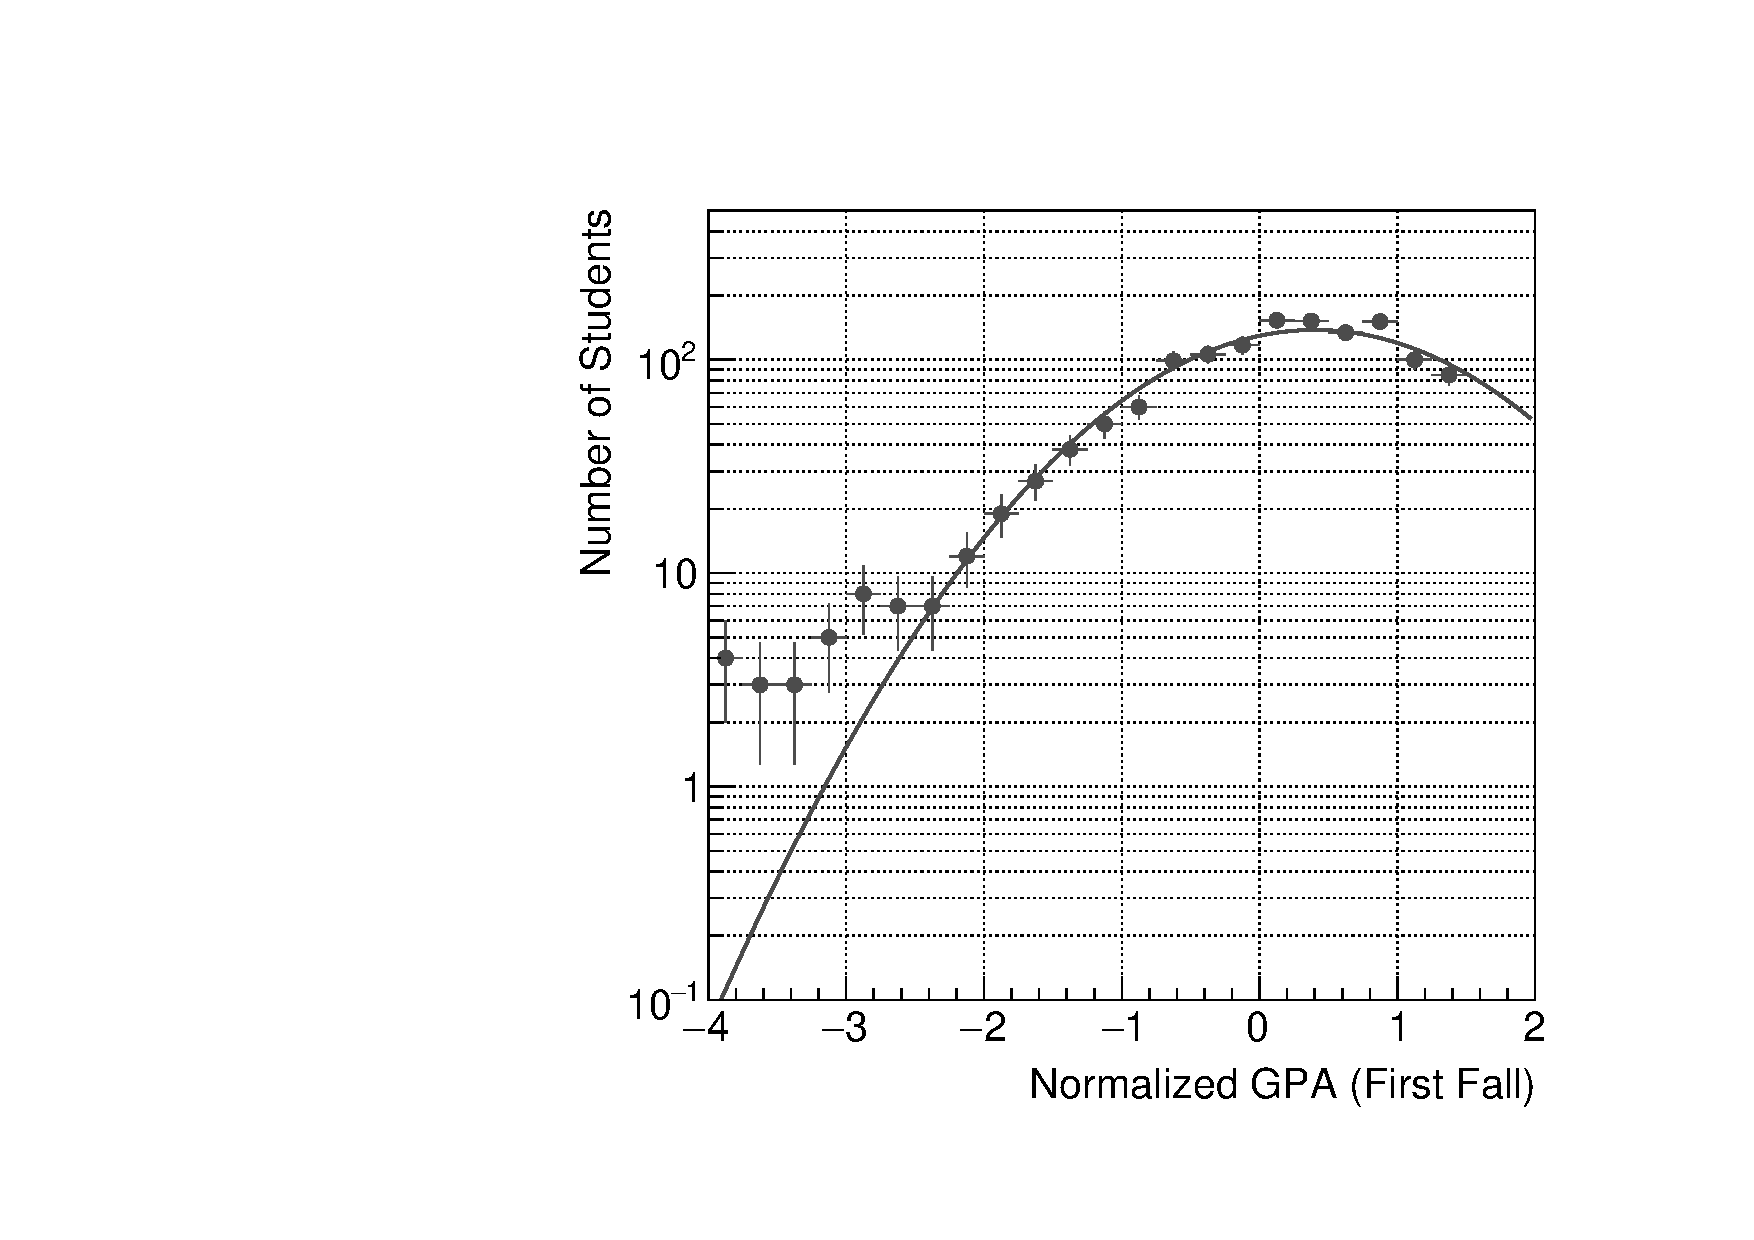
\includegraphics[width=0.4\textwidth]{figures/Nov15_plot3.pdf}
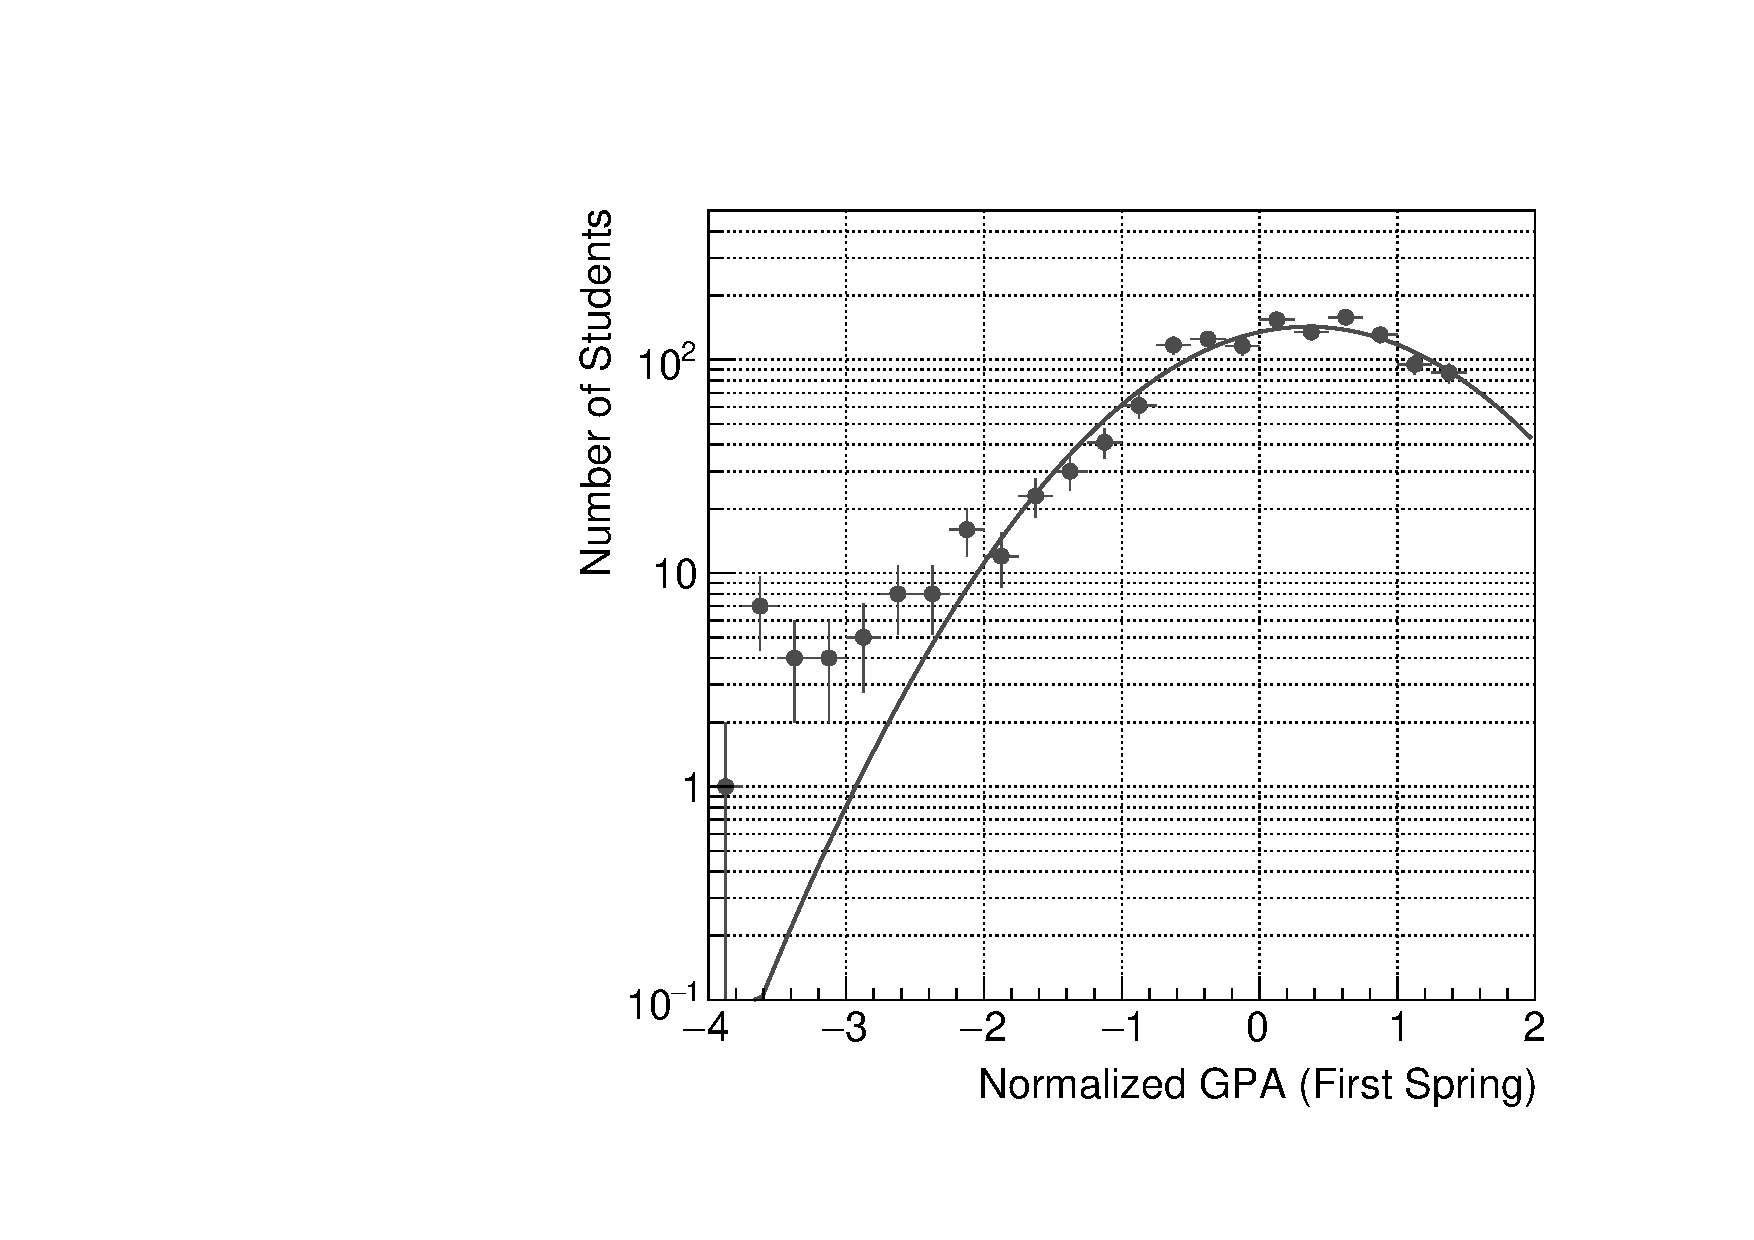
\includegraphics[width=0.4\textwidth]{figures/Nov15_plot9.pdf}
\caption{\label{fig:grade} (Left) A histogram of GPAs for 1,346 Whittier College students in the first semester.  (Right) Same, but for the second semester.}
\end{figure}

The next step was to try to identify the low-GPA students in advance using the data.  Decisions based on the findings would be by consensus, and with input from CAAS, athletics, and professors from all divisions.  My job was to find clues as to why we observed students receiving GPAs so far below the mean at a rate 10 times higher than expected.  I ran a series of statistical analyses, and I found that for students that \textit{do} proceed to the sophomore year, data from high school and college, and data from the first and second semester in college, is highly correlated.  For example, if we have the high school GPA of a student we know is going to proceed to sophomore year at Whittier College, we can predict first semester GPA at Whittier College accurately.  For students that we know do not proceed to sophomore year, the data yields no strong correlations.  I tried two machine learning methods to factor the data into statistical parameters that would reveal the difference between students that do and do not proceed.  The algorithms demonstrated only moderate success at classification. I felt there had to be more to the story.
\\
\vspace{0.15cm}
As part of the first analysis, I was fitting normal distributions to statistical data generated by our students.  One data column that came with the original files was named ``financial aid gap.''  As I understand it conceptually, a positive aid gap means that a student is receiving various forms of financial aid that total less than what they owe in tuition, after accounting for the expected family contribution\footnote{VP of Enrollment Management, Falone Serna, was kind enough to explain it to me in detail in my second year in ESAC, but during the first year this is essentially how I understood aid gaps.}.  I noticed that I could not explain the distribution of student financial aid gap with \textit{a single} normal distribution, and that a better fit was \textit{two normal distributions.}  Statistically speaking, the data sample is drawn from two distinct populations of students.  One had an average \textit{negative financial aid gap}, and the other had an average \textit{positive financial aid gap.}  One group was receiving aid and scholarships that exceeded their tuition, and another group was not.  This was the topic of my second ESAC presentation.
\\
\vspace{0.15cm}
I showed that aid gap is predicted by many things.  If a student has an SAT score (in any category) that is 1.5 or more standard deviations below the mean, then that student is almost always in the positive aid gap group.  The same is true for first and second semester GPAs.  If I graphed the aid gap distribution for just the students who did not proceed with sophomore year, a large fraction of those students were in the positive aid gap group (receiving less).  It is worth pointing out that the impetus for the analysis was Fig. \ref{fig:grade}.  Figure \ref{fig:grade2} contains the aid gap distribution.  What if the positive aid gap group and the low Whittier College GPA group were connected?  Figure \ref{fig:grade2} contains evidence of this.  However, I note that the data can be messy, and the proper claim is not simply that positive aid gap leads to low GPAs.  Rather, if a student receives a GPA of 1.5 standard deviations below the mean in the first semester, it is highly likely that the student has a positive aid gap.

\begin{figure}
\centering
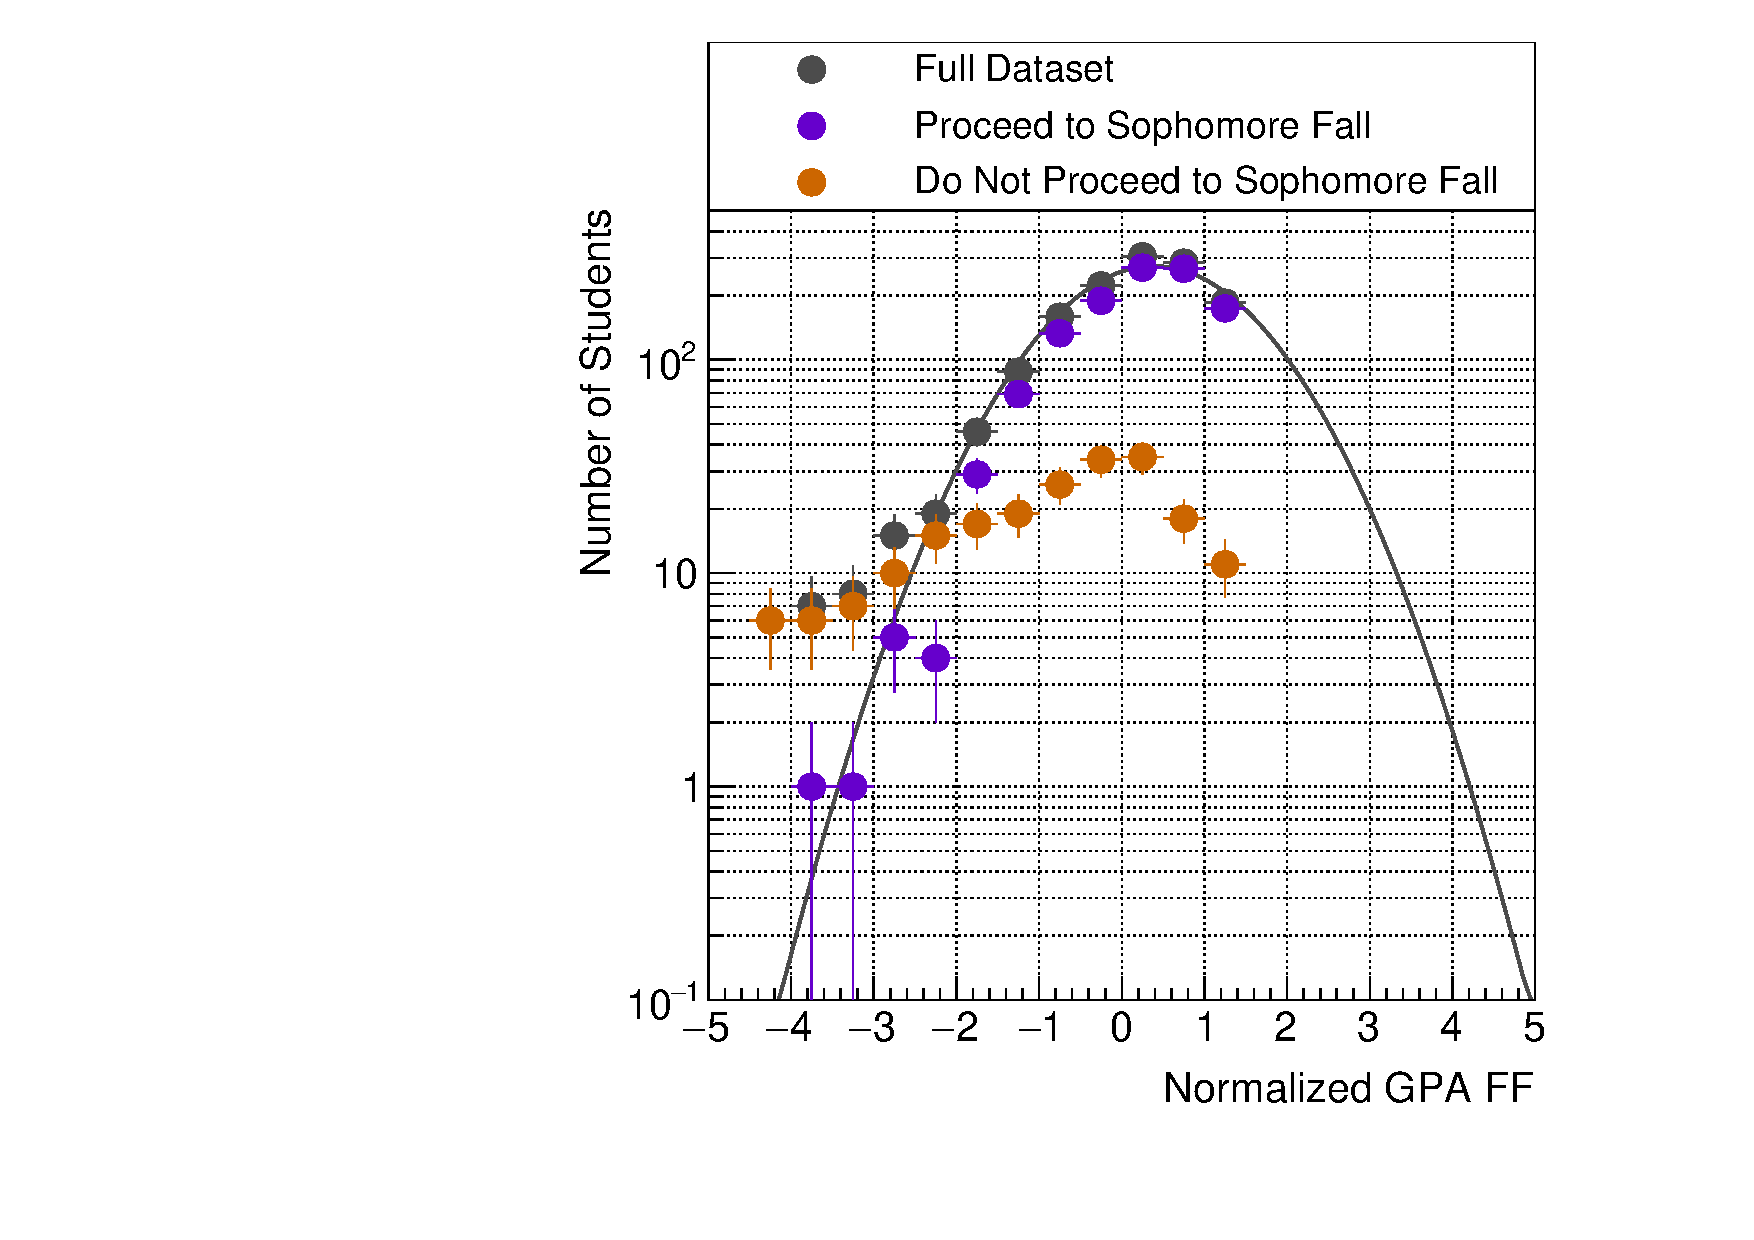
\includegraphics[width=0.4\textwidth]{figures/Dec5_plot6.pdf}
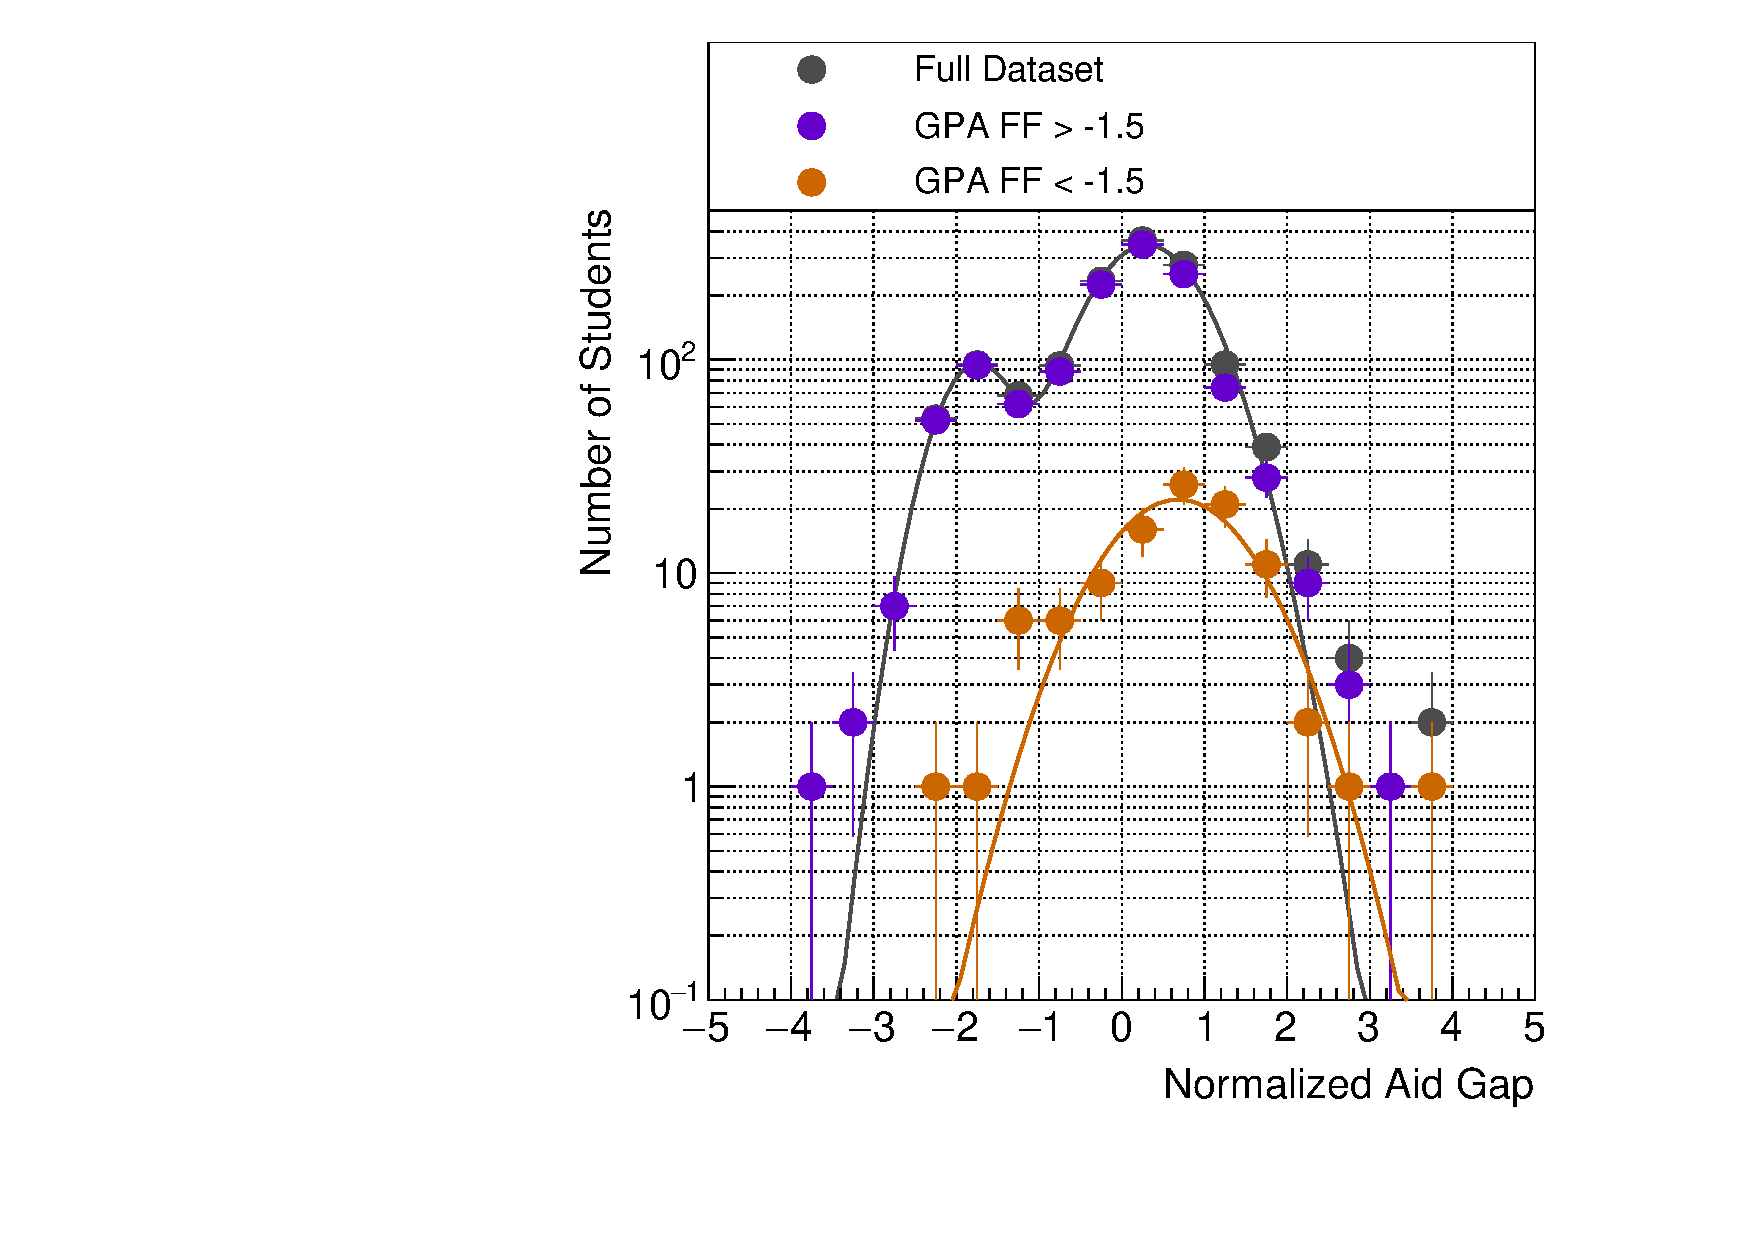
\includegraphics[width=0.4\textwidth]{figures/Dec4_plot5.pdf}
\caption{\label{fig:grade2} (Left) Histogram of normalized GPA for students' first fall semester for all students (black), those that proceed to sophomore year (purple), and those that do not (orange).  (Right) Same color scheme as (Left), but for aid gap.}
\end{figure}

\subsection{Educational Resources and Digital Liberal Arts Committee}

Our main achievement on the educational resources committee during 2020-21 was to create a policy and process for archival of senior thesis presentations.  We discussed a number of issues surrounding archival of senior projects.  First, there was the notion of quality control.  Some students take their senior projects very seriously, and treat the work as their first potential step into a professional world.  We created a form that documents the decision process for the entry of the senior project into the archive.  Both student and advisor must agree that the work is of sufficient quality.  Second, the student can control the searchability of their work.  A project may be visible to the broad internet, just those with access to Poet Commons, or simply archived but not visible for a period of time.  The period of time can be temporary or permanent.  This action protects the privacy and intellectual property of the student, while preserving their work for future members of the Poet community to understand.  Third, we included feedback from other committees regarding the structure of the form, and the implications of a decision now on the future visibility of a the senior project.

\subsection{Whittier Scholars Program}

Having served two years with ESAC and one with ERC/DLAC, I reflected this past semester on how my committee work could be the most productive for Whittier College.  I had experienced the Whittier Scholars Program (WSP) after advising a student to graduate through the program (see Sec. \ref{sec:advising_mentoring}), and felt that I could provide consistent, quality service to WSP.  In conversations with Prof. Andrea Rehn, director of WSP, I learned that working on the WSP advisory board is, on average, more work that most committees.  However, it is the \textit{type} of work that I can do well.  The main function of the WSP advisory board is to review student applications, which are educational roadmaps.  We interview students and advisors as a team, and get them to think carefully about the educational design given the intellectual landscape.  Providing intellectual and technical guidance from a liberal arts mindset is the type of service I can do well for Whittier College.
\\
\vspace{0.15cm}
With ESAC and the admissions criteria, for example, my impression was that the majority of our effort was spent in negotiation between people with different viewpoints.  Some thought absolutely no numerical limits to admissions criteria should be allowed, and some thought there must be some.  I performed my analysis as best I could while balancing my other responsibilities, but in the end the issue was resolved through political negotiation.  I agree that political negotiation was a necessary and diplomatic path forward, and we did end up developing a consensus.  However, others are much more adept at those negotiations than I am, and I think my analytical skill would be better utilized in other committees.  On the other hand, sometimes the administration needs us to help out where the help is needed, regardless of the type of work, and I am always open to serving where I am needed.
\\
\vspace{0.15cm}
I decided in Spring 2021 to inquire about serving WSP.  I spoke with Prof. Andrea Rehn, who excitedly welcomed me to join the WSP advisory board.  She added that it was a three-year service term, and I agreed that it made sense to have continuity.  Although it became official that I was to join the WSP program this Fall, we received word from the Faculty Executive Committee (FEC) that I was needed on the Educational Policies Committee (EPC) due to personnel issues.  \textit{I feel in this situation that it's important to be a team player}, knowing that there will be a time in the near future that I can serve WSP.  I am grateful to all of my committee chairs and fellow members for their hard work, and I look forward to serving in the future.

\end{document}
